%
% File: chap01.tex
% Author: Victor F. Brena-Medina
% Description: Introduction chapter where the biology goes.
%
\let\textcircled=\pgftextcircled
\chapter{Introduction}
\label{chap:intro}
\vspace{-0.2 cm}

\section{Motivation}

\paragraph{}

A paper, titled \textbf{The End of Moore's Law: A New Beginning for Information Technology[1]} by scholars from Stanford and Columbia University said that, "For the three decades prior to 2005, clock frequency, integration density, and cost per device all improved exponentially with each technology generation, while active and passive power were contained within economically acceptable bounds. Since 2005, integration density and cost per device have continued to improve, and manufacturers have emphasized the increasing number of processors (cores) and the amount of memory they can place on a single die. However, with clock frequencies stagnant, the resulting performance gains have been muted."

This paper emphasised on the challenges due to miniaturization of transistors and some other areas to think upon, from logic to computer architecture. Memory organizations like SRAM, DRAM, and NAND Flash were created to address workloads that had a more organised data locality. However the paper said, "such data movement is expensive in latency as well as energy consumption, especially when data need to come from off-chip memory through a data bus with limited bandwidth, Off-chip memory access can account for as much as 90 percent of energy and commensurate execution time in today’s computing systems running data-intensive algorithms."

\begin{figure}[h]
\begin{subfigure}{0.5\textwidth}
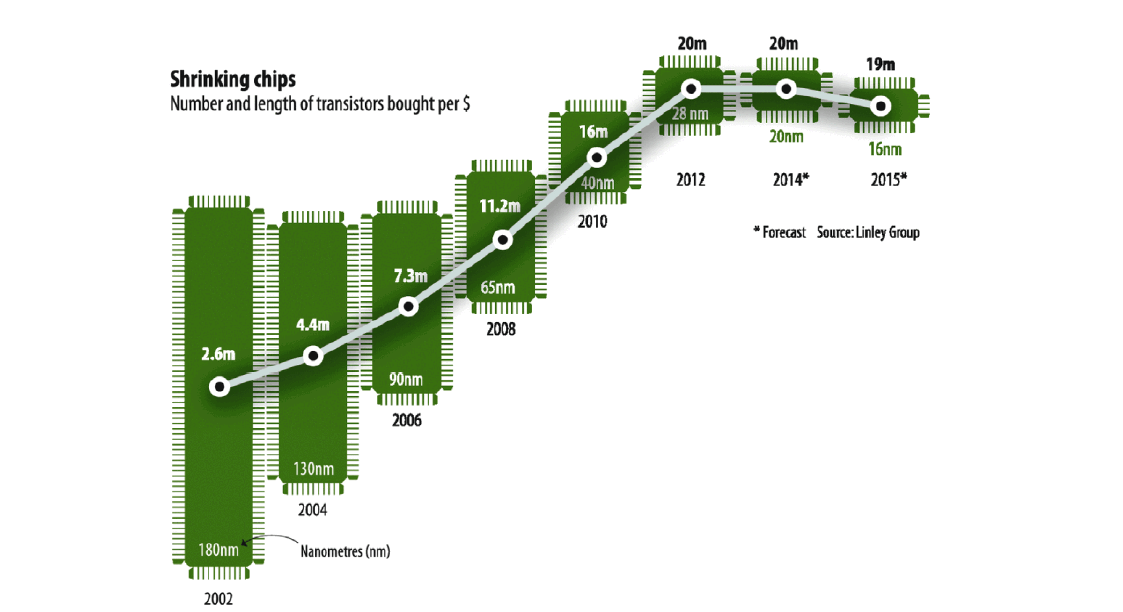
\includegraphics[width=0.9\linewidth]{chapters/chapter01/moore.png} 
\caption{Death of Moore's Law[1]}
\label{fig:Figure}
\end{subfigure}
\begin{subfigure}{0.5\textwidth}
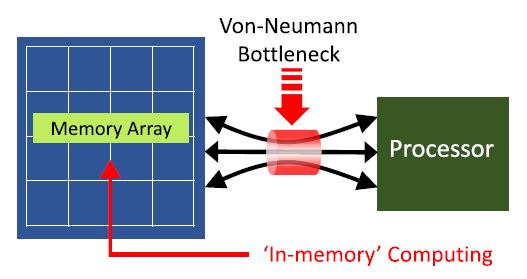
\includegraphics[width=0.9\linewidth]{fig1.JPG}
\caption{The Von-Neumann Bottleneck[2]}
\label{fig:Figure}
\end{subfigure}
 
\caption{Challenges for the current data centric world}
\label{fig:Figure}
\end{figure}


The current computing platforms are majorly based on the Von Neumann Bottleneck that contains decoupled Memory and Processor. Running data intensive applications on such systems in the current scenario of Artificial Intelligence boom, Big Data and advent of Internet of Things is limited by the Von-Neumann Bottleneck. Computational Speed for faster training \& analysis and Low Power devices for IOT are the major out of many issues with this bottleneck. 

Thus innovation in Nanometer Devices or new architectural and circuital designs of the computer are ways that can breakthrough this barrier. One of the most promising approach is \textbf{In Memory Computation}, which aims to embed logic inside the memory for reduced data transfers with less area and power consumption.

\begin{figure}[htbp!]
\centering
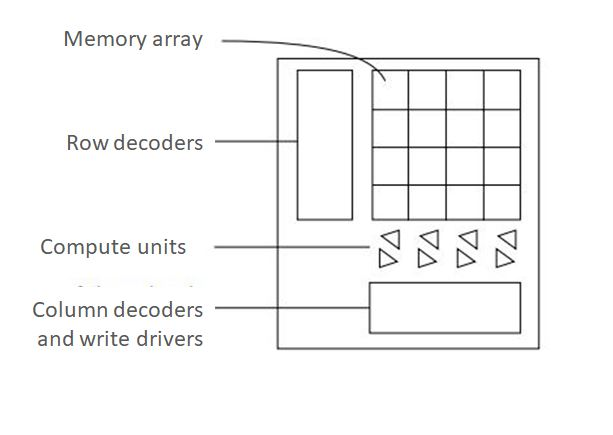
\includegraphics[width=0.7\textwidth]{fig2.JPG}
\caption{Idea behind In-Memory Computation}
\label{fig:Figure}
\end{figure}

The picture painted by the In Memory Computation architecture is somewhat like conventional memory organization, with decoders, write drivers, pre-charge circuitry around the memory array but with these peripherals only slightly modified and an included computational unit which is designed in a new way to adjust it near the memory array so that less area is taken up, by ensuring to use less of conventional digital circuits. As of now these architectures are application specific, the logic and peripherals embedded with the memory array are subject to task being performed and efforts are being made to make these architectures more and more generic.  

\section{Problem Definition}

\paragraph{}

The aim of this thesis is to design an Architecture for In-memory Computation such that area is optimised along with substantial amount of operations that can be performed to carry out numerous tasks. The steps taken in this regard are as follows:
\begin{itemize}
  \item Using 8T-SRAM cells due to their decoupled read and write ports.
  \item Taking advantage of the decoupled read port in order to perform logical operations without using conventional gates that take up more area.
  \item Designing arithmetic blocks and operations like Shift Left and Right to perform mathematical operations. 
  \item Designing memory peripherals according to our new architecture to allow reading at most two operands, computing the result and storing the result at the desired location.
  \item Along with computation, basic memory read, write will also be a functionality with an addition of copy operation from one word to other.
  \item Simulation of the whole design using an Assembly program in order to ease the usage of the proposed design. 
  \item The above task will require an Assembler code to convert the Assembly code to Machine code i.e stream of bits which will be used as control signals for the circuitry.
  \item Keeping in mind the scope for scalabilty and ease of modification while designing the memory array, compute blocks and peripheral circuits.
\end{itemize}

\section{Contributions}
\paragraph{}
The objective of this thesis is to design a basic architecture for In-Memory computation that can have operations essential to many tasks. In designing the circuits for the architecture, new methods for logical operations using the read line of 8T SRAM and shifting a word without the use Flip Flops have been developed.

\section{Thesis Organization}
\paragraph{}
\textbf{Chapter 1} gives an introduction to the problem along with the motivation and need for ideas like In Memory Computation to get rid of the Von-Neumann Bottleneck in the current scenario.

\textbf{Chapter 2} throws some light upon the work in the area of In-Memory computing already done and the current scenario of it's increasing development by research scholars and companies. 

\textbf{Chapter 3} discusses the basic building block, the 8T SRAM cell, reason for considering it over the conventional 6T SRAM and the read and write stability of 8T SRAM.

\textbf{Chapter 4} discusses the design of logical and arithmetic blocks, how the design reduces area and how are they implemented along with 8T SRAM.

\textbf{Chapter 5} discusses the peripherals that have been designed for our memory array to support computation and storage in the memory itself.

\textbf{Chapter 6}  provides a complete picture with all the components in place and the execution cycle that takes place in accordance with the control signals that are generated by the assembly code.

\textbf{Chapter 7}  takes a look into the results of simulation, delay and power consumption by the proposed design.

\textbf{Chapter 8}  concludes this thesis and provides the inferences drawn from this project along with future scope and developments.


